\paragraph{Sơ đồ tuần tự luồng Xác nhận liên kết từ Email (Email Link Verification \& Redirect)}

Luồng nghiệp vụ này mô tả
quá trình xác thực token
khi người dùng click
vào liên kết khôi phục trong email,
nhận phiên đăng nhập từ callback
và tiếp tục qua bước MFA trước khi
được chuyển tới trang đổi mật khẩu của ứng dụng.

\begin{figure}[H]
\centering
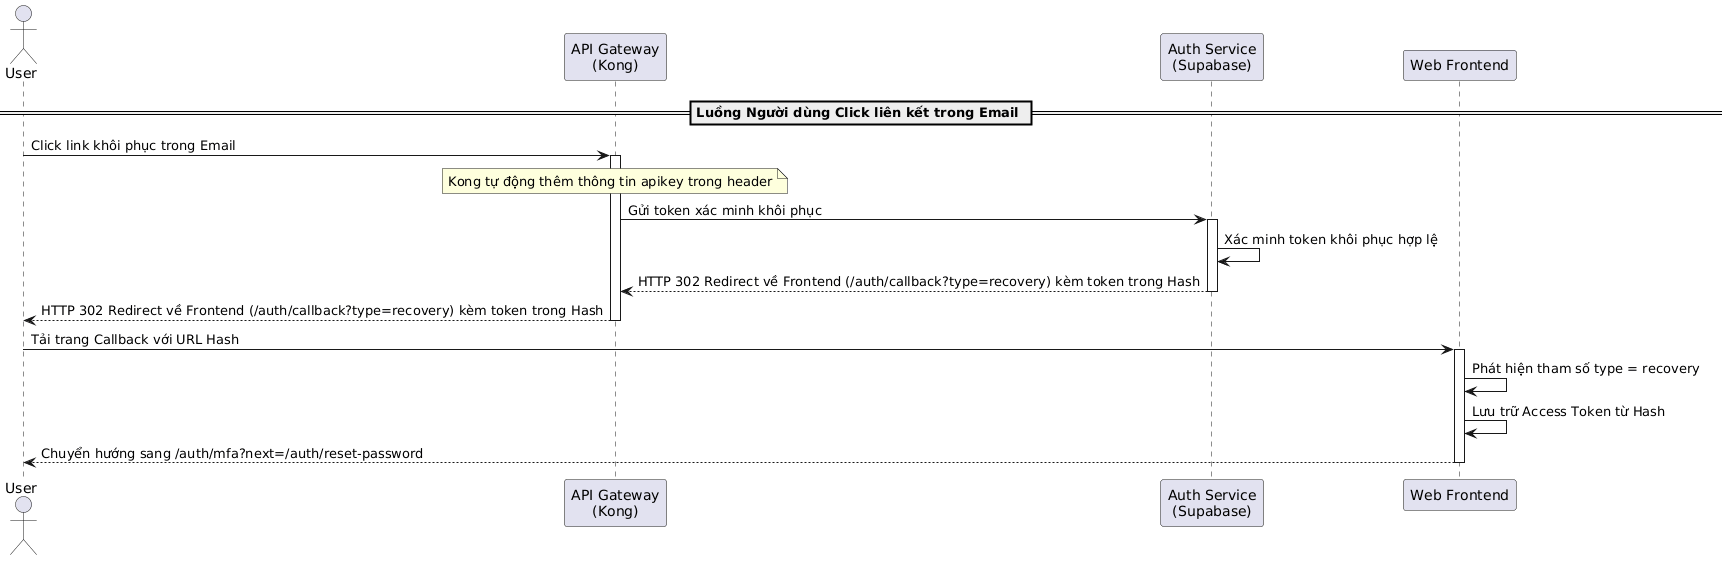
\includegraphics[scale = 0.2]{contents/Sequence/UML-Sequence-UserEmailLinkVerificationRedirect.png}
\caption{Sơ đồ tuần tự luồng Xác nhận liên kết từ Email}
\end{figure}

\subparagraph{Các thành phần tham gia}

\begin{table}[H]
\centering
\renewcommand{\arraystretch}{1.3}

\begin{tabular}{|l|l|p{5cm}|}
\hline
\textbf{Thành phần} & \textbf{Phân loại} & \textbf{Vai trò trong hệ thống} \\ \hline
User & Actor & Người dùng click liên kết xác nhận. \\ \hline
API Gateway (Kong) & Component & Cổng API chuyển tiếp các yêu cầu API. \\ \hline
Auth Service (Supabase) & Microservice & Dịch vụ Supabase Auth xác minh token khôi phục và trả về HTTP 302 Redirect. \\ \hline
Web Frontend & Component & Giao diện web Next.js. \\ \hline
\end{tabular}
\caption{Các thành phần tham gia luồng Xác nhận liên kết từ Email}
\end{table}

\subparagraph{Mô tả tổng quan}

\begin{itemize}
\item Người dùng click vào link trong email. Yêu cầu chuyển qua Kong Gateway tới Auth Service để tự thực hiện xác minh tính hợp lệ của token.
\item Nếu hợp lệ, Auth Service trả về HTTP 302 Redirect hướng trình duyệt của người dùng đến địa chỉ \texttt{/auth/callback?type=recovery} của Web Frontend kèm theo token tạm trong URL Hash.
\item Frontend nhận callback, lưu trữ token từ Hash và chuyển hướng người dùng sang trang đổi mật khẩu, sau khi hoàn tất MFA, hệ thống mới điều hướng tới trang đặt lại mật khẩu.
\end{itemize}
